\documentclass[10pt,a4paper]{article}
\usepackage[utf8]{inputenc}
\usepackage[italian]{babel}
\usepackage{amsmath}
\usepackage{amsfonts}
\usepackage{amssymb}
\usepackage{graphicx}
\usepackage{gensymb}
\usepackage[left=2cm,right=2cm,top=2cm,bottom=2cm]{geometry}
\newcommand{\rem}[1]{[\emph{#1}]}

\author{Gruppo BN \\Lisa Bedini,  Federico Belliardo, Marco Costa}
\title{Esperienza 13: Semaforo}

\begin{document}
\maketitle

%TODO - Secondo me in tutta la relazione le immagini non sono il massimo avrei voluto mettere le immagini del flip-flop congelato, ma non le abbiamo prese. Le immagini che mostrano le misure dei tempi non sono il massimo. Io le toglierei.

\section{Scopo dell'esperienza}
Lo scopo dell'esperienza è di realizzare un semaforo come macchina a stati finiti tale che
\begin{itemize}
\item nello stato ENABLED esegua un ciclo in cui si abbiano accesi (per la durata di un colpo di clock e nel seguente ordine) Led Verde, Led Verde e Giallo, Led Rosso.
\item nello stato NOT ENABLED faccia lampeggiare il Led Giallo (sincronamente  col clock).
\end{itemize}
Il semaforo è stato realizzato sia tramite circuiti integrati, sia programmando Arduino.

\section{Materiale a disposizione}
%correggi
\begin{itemize}
\item 2 SN7474 Dual D-FlipFlop
\item 1 SN7400 Quad NAND gate
\item 1 SN7408 Quad AND gate
\item 1 7432 Quad OR gate
\item DIP switch
\item 3 Led: verde, giallo, rosso
\end{itemize}
%I valori delle componenti sono state misurate con multimetro digitale (incertezza riportata sul manuale).
%Le differenze di potenziale sono state misurate tramite oscilloscopio, se non indicato diversamente, e come incertezza si è presa la sensibilità dei cursori più il 3\% di calibrazione.
%Per misurare i tempi si è usato l'oscilloscopio e come relativa incertezza si è preso il massimo fra la sensibilità dei cursori e la semidispersione dei valori plausibili.

\section{Stato Enabled}

Per realizzare il solo stato enabled abbiamo optato per una macchina di Moore, non essendoci alcun tipo di input. I tre stati della macchina sono 'Verde', 'Verde e Giallo', 'Rosso'. Abbiamo deciso di usare solo 2 FF in quanto due bit erano sufficienti per codificare i tre stati richiesti. Indicheremo sempre (anche nei punti successivi della relazione) $Q_1$ il bit più significativo, mentre $Q_0$ sarà sempre il bit meno significativo della codifica. In figura \ref{fig:FSMenabled} abbiamo disegnato le transizioni e la codifica dei vari stati.
\begin{figure}[!htb]
\centering
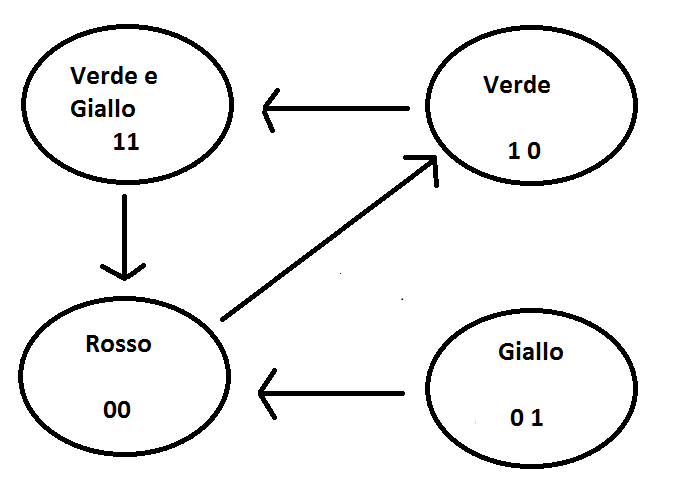
\includegraphics[scale=0.7]{FSMenabled.png}
\caption{Diagramma dello stato Enabled. Le transizioni avvengono aad ogni colpo di clock.\label{fig:FSMenabled}}
\end{figure}
%In arrivo ftrase ambigua
Abbiamo deciso di codificare lo stato rimanente (10 in termini di bit) come lo stato in cui il solo Led Giallo è acceso. Tale stato compare nel circuito solo nella eventualità in cui i FF si accendano in questo stato. Salvo in questo caso, 01 non compare più nei cicli successivi.
Il vantaggio di questa codifica è che il Led Verde e il Led Giallo sono pilotati da due bit distinti, rispettivamente $Q_1$ e $Q_0$ nel nostro caso. In questo modo ci sarà più facile in seguito poter far lampeggiare il solo Led Giallo.
Le tabelle di transizione implementate sono riportate in tabella \ref{tab:transiozioneenabled} (I don't care sono stati assegnati in questa tabella: nelle sezioni successive diamo una breve spiegazione su come sono stati eliminati).
\begin{table}[!htb]
\centering
\begin{tabular}{|c|c|c|c||c|c||c|c|c|}
\hline
$Q_{1,n}$ & $Q_{0,n}$ & $D_{1, n}$ & $D_{0, n}$& $Q_{1,n+1}$ & $Q_{0,n+1}$ & $LV$ & $LG$ & $LR$\\
\hline
0 & 0 & 1 & 0 & 1 & 0 & 0 & 0 & 1 \\
0 & 1 & 0 & 0 & 0 & 0 & 0 & 1 & 0\\
1 & 0 & 1 & 1 & 1 & 1 & 1 & 0 & 0\\
1 & 1 & 0 & 0 & 0 & 0 & 1 & 1 & 0\\
\hline
\end{tabular}
\caption{Tabella di verità delle transizioni fra stato $n$ e il successivo $n+1$, e delle uscite (in funzione dello stato $n$).\label{tab:transizioneenabled}}
\end{table}
\subsection{Funzioni logiche delle transizioni}
Nella funzione di transizione, abbiamo libertà di scegliere la transizione dello stato 'Giallo' 01.
Con un rapido studio tramite mappe di Karnaugh ci si convince facilmente che ponendo i due don't care\footnote{In realtà non sono prorpiamente dei don't care: è' lecito assegnare a questi  tutte le combinazione tranne 01, caso in cui la macchina resterebbe perpetuamente in questo stato.} pari a 0 si ottiene che la funzione richiesta è \begin{equation}
Q_{1, n+1} = \bar{Q}_{0,n}\qquad Q_{0,n+1} = \bar{Q}_{0,n}\cdotQ_{1,n} 
\end{equation}
Così si ha che lo stato non richiesto 01 ("solo giallo acceso"), transisce nello stato 00 ("solo rosso acceso").
Dato che abbiamo dei FF di tipo D, il valore di $Q_{i, n+1}$ è uguale al valore dell'ingresso $D_i$ nello stato $n$: minimizzare quindi le funzioni logiche dei $Q_{i,n+1}$ effettivamente minimizza il numero di porte logiche da implementare fisicamente.
\subsection{Funzioni logiche delle uscite}
Una volta codificati gli stati, abbiamo assegnato alle uscite $L_V$ (Led Verde), $L_G$ (Led Giallo), $L_R$ (Led Rosso) i seguenti valori:
\begin{equation}
L_V = Q_1 \qquad L_G = Q_0 \qquad L_R = \bar{Q}_0\cdot \bar{Q}_1
\end{equation}
Questo era in effetti il modo più semplice per realizzare i collegamenti fra i FF e le uscite: per come erano stati codificati gli stati, i Led Verde e Giallo sono pilotabili direttamente dal rispettivo bit, mentre per il Led Rosso abbiamo scelto l'unica funzione che valga 1 solo sullo stato 00. %In effetti avremmo pure potuto prendere come funzione per pilotare il Led rosso $\bar{Q_1}$, a patto però di avere 01 stato in cui sia il giallo che il rosso sono accesi. Abbiamo preferito usare una porta in più qui e avere la possibilità di controllare il Led giallo direttamente.
% e ce credo, erano davvero una cazzata...
%non mi piace come è scritta questa parte: ad esempio all'inizio dico subito che lo stato 0 1 è il giallo ma solo ora dichiao in effetti a cosa sia collegata l'uscita L_G... Inoltre, sebbne la tabella di transizione la ho scritta bene, devo far capire che poi i q_n+1 sarebbero gli ingressi D...
\subsection{Implementazione del circuito}
Abbiamo implementato il circuito come in figura\ref{fig:circenable}.
Abbiamo collegato i clear e reset dei FF a $V_CC = 4.9\pm0.1 $V tramite resistenze di pull-up di resistenza circa $1.5\mbox{k}\Omega$.
Abbiamo collegato i Led a terra tramite resistenza da circa $330\Omega$ per limitare la corrente.  
Abbiamo preso le forme d'onda di Clock e ciascuno dei tre Led tramite oscilloscopio.
\begin{figure}[!htb]
\centering
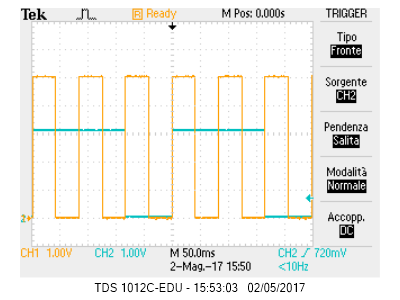
\includegraphics[scale=0.7]{clock-verde.png}
\caption{In CH1 il segnale del clock, in CH2 quello del Led Verde.\label{fig:verde}}
\end{figure}

\begin{figure}[!htb]
\centering
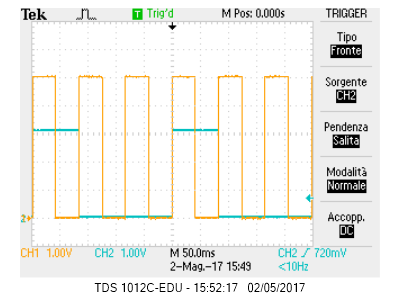
\includegraphics[scale=0.7]{clock-gialloverde.png}
\caption{In CH1 il segnale del clock, in CH2 quello del Led Giallo.\label{fig:giallo}}
\end{figure}

\begin{figure}[!htb]
\centering
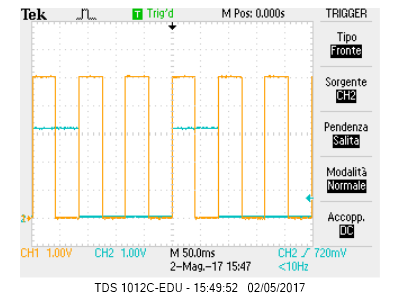
\includegraphics[scale=0.7]{clock-rosso.png}
\caption{In CH1 il segnale del clock, in CH2 quello del Led Rosso.\label{fig:rosso}}
\end{figure}
Si osservi che i segnali dei Led (e quindi delle uscite dei FF, a meno di ritardi trascurabili) diventano positivi quando il clock è sul fronte positivo (abbiamo edge-positive triggered Flip-Flop).
Inoltre, come atteso, si osserva che il Led Giallo e Rosso stanno accesi per un periodo di clock e spenti per i due successivi (Figure \ref{fig:giallo} e \ref{fig:rosso}), mentre il Verde il contrario (Figura \ref{fig:verde}).

\section{Semaforo completo}
Abbiamo scelto di usare una macchina di Mealy per realizzare il semaforo completo. Si è mantenuta la stessa codifica degli stati in termini di bit utilizzata precedentemente. In questo modo la funzione di transizione nello state Enabled è identica a quella precedente. Abbiamo chiamato E il valore logico dell'enable.
Abbiamo deciso di scegliere lo stato Enabled attivo alto (ossia quando $E = 1$):%spiega perchè
In tabella \ref{tab:semaforocompleto} abbiamo le transizioni e i valori delle uscite implementata (i don't care sono stati assegnati), mentre in figura \ref{fig:FSMcomplete} abbiamo disegnato la mappa delle transizioni (nella figura gli output sono stati codificati nell'ordine LV-LG-LR)
\begin{figure}[!htb]
\centering
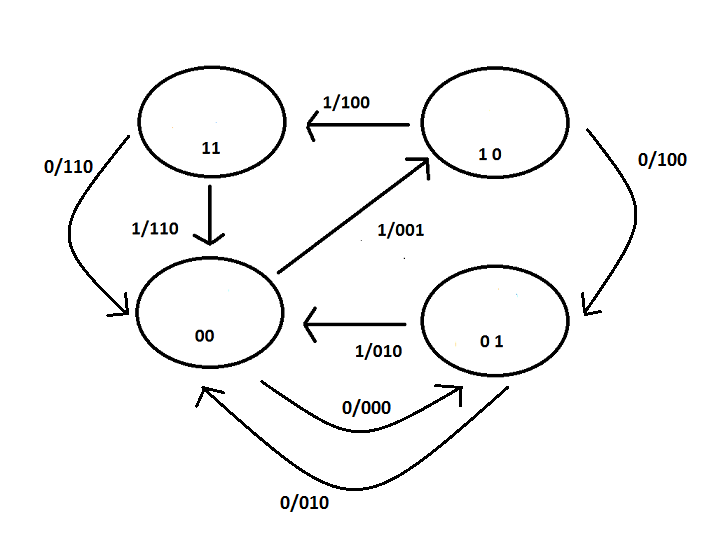
\includegraphics[scale=0.7]{FSMcomplete.png}
\caption{Diagramma delle transizioni per la macchina di Mealy realizzata. La terna degli output è LV-LG-LR.\label{fig:FSMcomplete}}
\end{figure}
\begin{table}
\centering
\begin{tabular}{|c||c|c|c|c||c|c||c|c|c|}
\hline
$E$ & $Q_{1,n}$ & $Q_{0, n}$ & $D_{1,n}$ & $D_{0,n}$ & $Q_{1, n+1}$ & $Q_{0, n+1}$ & $LV$ & $LG$ & $LR$\\
\hline
0 & 0 & 0 & 0 & 1 & 0 & 1 & 0 & 0 & 0 \\
0 & 0 & 1 & 0 & 0 & 0 & 0 & 0 & 1 & 0\\
0 & 1 & 0 & 0 & 1 & 0 & 1 & 1 & 0 & 0\\
0 & 1 & 1 & 0 & 0 & 0 & 0 & 1 & 1 & 0\\
\hline
1 & 0 & 0 & 1 & 0 & 1 & 0 & 0 & 0 & 1 \\
1 & 0 & 1 & 0 & 0 & 0 & 0 & 0 & 1 & 0\\
1 & 1 & 0 & 1 & 1 & 1 & 1 & 1 & 0 & 0\\
1 & 1 & 1 & 0 & 0 & 0 & 0 & 1 & 1 & 0\\
\hline
\end{tabular}
\caption{Matrice di transizione e valori di verità per le uscite nel caso di semaforo completo. (Uscite funzione dello stato $n$) \label{tab:semaforocompleto}}
\end{table} 
\subsection{Funzioni logiche delle transizioni}
Nel caso Not Enabled, abbiamo deciso di mantenere lo stato 01 ad essere con solo il Led Giallo acceso. Abbiamo deciso di farlo transire verso 10 : in modalità Enabled lo stato 00 aveva solo il Led Rosso acceso, pertanto con una aggiunta di un AND con il bit E si è riusciti a mantenere il circuito già montato in precedenza. Le transizioni degli altri stati (10 e 11) sono state scelte in modo che le relative mappe di Karnaugh risultassero le più semplici possibili compatibilmente col fatto che gli stati 10 e 11 non devono permanere mai nel ciclo.
Abbiamo così ottenuto come funzioni logiche per le transizioni:
\begin{equation}
Q_{0, n+1} = \bar{Q}_{0,n}\cdot(\bar{E}+Q_{1,n})\qquad
Q_{1, n+1} = E\cdot \bar{Q}_{0, n}
\end{equation}
\subsection{Funzioni logiche delle uscite}
Con lo stesso modo si sono scelte le funzioni di output dei Led relativamente ai soliti stati indesiderati 11 e 10. Stavolta i valori logici degli output sono dei veri don't care (possiamo effettivamene asseganre ad essi qualsiasi valore logico). Abbiamo ottenuto le seguenti equazioni:
\begin{equation}
LV = Q_1\qquad LG = Q_0\qquad LR = E\cdot(\bar{Q}_1\cdot\bar{Q}_0)
\end{equation}
Si osservi che il Led Verde in teoria può essere acceso nello stato Not Enabled, ma questo può accadere solo se la macchina viene inizializzata in uno di quegli stati, poi dopo la prima transizione resta sempre spento SE $E=0$%spiega meglio?

\subsection{Implementazione del circuito}
Abbiamo implementato il circuito in figura \ref{fig:circ}.
%figura circuito con piedini numerati
Si osservi che in questo caso abbiamo implementato un meccanismo di abilitazione asincrona: non appena si cambia lo stato di $E$, indipendentemente dal fronte del clock, si ha che il semaforo cambia stato di abilitazione.
Dalla figura \ref{fig:circ} si può in effetti vedere che il passaggio di $E$ da 1 a 0 disabilita istantaneamente la porta AND che precede il Led Rosso. Pertanto se si è nello stato enabled $E=1$ a $E=0$ mentre è acceso il Led Rosso, si ha un immediato suo immediato spegnimento (e quindi si hanno tutte le uscite con valore logico 0). Si osservi tuttavia che lo stato dei FF non è cambiato: questi cambiano solo dopo un colpo di clock.
In figura \ref{fig:lampeggiante} possiamo osservare come nello stato Not Enabled il Led Giallo si accenda e si spenga il periodo di clock successivo.
\begin{figure}
\centering
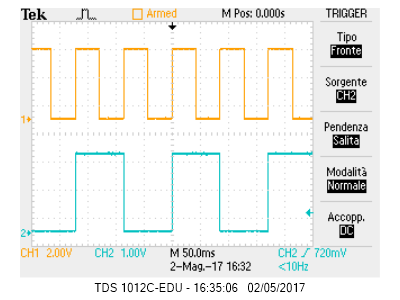
\includegraphics[scale=0.7]{ch1clock-ch2giallolamp.png}
\caption{In alto il sengale del clock, in basso l'uscita al Led Giallo in modalità Not Enabled\label{fig:lampeggiante}}
\end{figure} %Il Led Rosso è collegato all'enable non tramite altri D-Latch, quindi  se è acceso mentre $E$ passa da 1 a 0, avviene immediatamente il cambio dei valori logici delle uscite previste nel caso di $E = 0$, ossia si passa all'uscita $LG=1$ senza aspettare il clock.
%Per le altre uscite non ci sono problemi in quanto sono collegate ad $E$ solo tramite i vecchi D-Latch.
\subsection{Abilitazione sincrona}
Per realizzare un meccanismo di abilitazione sincrona, ossia per fare in modo che il semaforo registri solo cambiamenti di $E$ che avvengono sul fronte alto del clock, si è collegato $E$ all'AND che lo porta al Led Rosso (che causava cambi di output istantanei) tramite un terzo D-Latch, come in figura\ref{fig:sincrono}.
E' sufficiente l'aggiunta di questo solo FF perchè gli altri due collegamenti che si hanno con l'Enable sono verso gli ingressi D dei FF, che registrano i cambiamenti degli input in modo sincrono.
%Si osservi che a differenza di prima, si osserva una transizione diversa se passiamo da Enabled a Not Enabled quando ci troviamo nello stato 00 (Led Rosso acceso); nel circuito costruito prima si passa subito a stato spento 00, che poi transisce a 01 (ossia con il solo Led Giallo acceso). Adesso si ha una transizione a 10, in cui si ha il Led Verde acceso, e poi si entra nel ciclo 00/01, in cui si ha il Led Giallo lampeggiante.
\section{Semaforo con Arduino}
Adesso vogliamo implementare lo stesso semaforo programmando Arduino. Abbiamo optato per una macchina di tipo Moore, più semplice concettualmente da realizzare.
Abbiamo collegato le uscite di Arduino 9, 10, 11 tramite il buffer rispettivamente ai Led Verde, Giallo, Rosso, inserendo resistenza da $330\Omega$ su ciascuno per limitare la corrente.
Queste uscite sono state dichiarate come OUTPUT nel programma utilizzato.
L'enable è stato collegato all'uscita 8, e nel programma è dichiarato come INPUT-PULLUP (ossia alto se interruttore aperto e basso se chiuso).
Dato che con Arduino si hanno in genere un numero di bit a sufficienza, nello scrivere il programma abbiamo assegnato ad ogni Led un bit diverso. In questo modo si ha uno stato per ogni Led acceso, più lo stato spento e lo stato in cui Verde e Giallo sono accesi. Abbiamo considerato solo i vari stati che ci servono: quelli indesiderati non si presentano mai dato che l'inizializzazione (nello stato in cui tutto è spento) viene fatta da noi nel programma e non casualmente come nel caso dei FF.
Il funzionamento del programma mima il comportamento della macchina a stati finiti precedentemente costruita:
\begin{itemize}
\item Legge il valore dell'Enable (attivo alto)
\item Legge lo stato in cui si trova attualmente
\item Calcola lo stato successivo in cui andare a seconda dello stato attuale e del valore di Enable
\item Accende i Led relativi allo stato in cui si trova la macchina (E' di tipo Moore, quindi lo stato determina le uscite) per il tempo impostato
\item Dopo l'attesa, ripete il ciclo dall'inizio
\end{itemize}
Si osservi che in questa macchina si ha una abilitazione sincrona (avviene solo ad inizio ciclo la lettura dell'input)

\section{Conclusioni}
Abbiamo realizzato una macchina a stati finiti secondo le specifiche richieste.
Si è realizzato un meccanismo di Enable sia asincrono che sincrono.
Non sono state riscontrate deviazioni del comportamento dei circuiti costruiti rispetto a quanto atteso nel caso di macchina ideale.
\end{document}







